\scanpage{23}
au fond où $\mathcal C$ serait la formalisation de la catégorie triviale définie par $X_0/\mathrm{Spec}\,\mathbb Z$). En particulier
\[
\mathfrak g^{\mathcal C}=\deleted{\unsure{\mathrm{dual}|\text{déf}|\text{dér}}}\ \underline{\mathrm{Hom}}_{\underline O_{X_0}}(\Omega_{\mathcal C}^{\deleted{\unsure{\mathcal C}}},\underline O_X)=\varinjlim_{\alpha}\underline{\mathrm{Hom}}_{\underline O_{X_0}}(\Omega_{G_\alpha}^{\mathcal C},\underline O_{X_0})
\]
opère sur $\underline O_{X_0}$ par \uline{dérivations}..... Cf aussi plus bas pour sa déduction à partir du complexe de De Rham $\Omega_{\mathcal C}^{*\deleted{\unsure{\mathcal C}}}$ de $\mathcal C$.

2.\quad \uline{Complexes de De Rham} \uline{généraux}.

Appelons complexe de De Rham construit sur un \deleted{sch\unsure{é}} Module \begin{tabular}[b]{@{}l@{}}\inserted{\unsure{qu.|q.} coh}\\[-0.8ex]\begin{tikzpicture}[x=1cm,y=0.5cm,baseline]\draw (0,0) .. controls (-.04,.15) and (.28,.55) .. (.69,.7) .. controls (1.07,.86) and (1.44,.99) .. (1.41,1.15);\end{tikzpicture}\end{tabular} $\Omega$ sur un sché\unsure{m|ma}. $X_0$ [NB marchera aussi pour tout espace annelé, de $\unsure{\overline{\mathrm m}|=}$ que les sorites de 1.] \begin{tabular}[b]{@{}l@{}}
\inserted{tout complexe obtenu par}\\[-0.8ex]
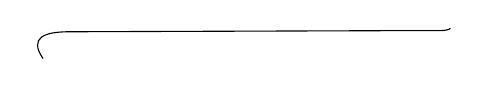
\begin{tikzpicture}[x=0.75cm,y=0.5cm,baseline]
\draw (0,0) .. controls (-0.25,0.55) and (0.05,0.67) .. (0.4,0.68) -- (6.25,0.71) .. controls (6.7,0.71) and (6.85,0.69) .. (6.9,0.77);
\end{tikzpicture}
\end{tabular} une \deleted{\unsure{o}p} différentielle d'anneau gradué sur $\overset{*}{\bigwedge}\Omega$.

\uline{Remarque} 1\quad Cette différentielle est connue quand on la connaît en degrés 0 et 1
\[
\begin{aligned}
\delta_0:\underline O_{X_0}\longrightarrow\Omega\quad &\begin{gathered}[b]
\inserted{\alpha)\ \text{\uline{dérivation}}}\\[-0.8ex]
\text{\begin{tikzpicture}[x=0.8cm,y=0.5cm,baseline]\draw (.04,0) .. controls (-.12,.3) and (.2,.53) .. (.61,.6) .. controls (1.0,.68) and (1.14,.71) .. (1.30,.73); \draw (1.36,.74) .. controls (1.75,.77) and (2.2,.80) .. (2.55,.91) .. controls (2.96,1.03) and (3.11,1.2) .. (3.09,1.25) .. controls (3.07,1.3) and (3.02,1.28) .. (2.98,1.24);\end{tikzpicture}}
\end{gathered}\quad [\,\text{i.e.}\quad\Omega^1_{X_0/\mathbb Z}\xrightarrow{u}\Omega\\
\inserted{\unsure{\alpha|\alpha'})\ \delta_0(fg)=\delta_0(f)g+f\delta_0(g)}\quad &\text{par}\quad\delta(f)=u(df)\quad]\\
\delta_1:\Omega\longrightarrow\overset{2}{A}\Omega &
\end{aligned}
\]

Condition nécessaire sur $\delta_1$
\[
\begin{array}{@{}c@{\quad}l@{}}
\vcenter{\hbox{\begin{tikzpicture}[x=1cm,y=0.5cm]\draw[line width=.4pt] (0,2.8) .. controls (-.01,2.53) and (.03,2.3) .. (.08,2.1); \draw[line width=.3pt] (.08,2.0) .. controls (.11,1.7) and (.18,1.4) .. (.22,1.1); \draw[line width=.5pt] (.22,1.02) .. controls (.21,.69) and (.26,.32) .. (.31,0); \draw[line width=.4pt] (-.15,2.23)--(-.08,2.1); \draw[line width=.4pt] (-.03,1.97)--(.08,1.9);\end{tikzpicture}}}
&\begin{aligned}
\unsure{\beta'|\beta})\quad&\delta_1(f\omega)=\delta_0(f)\,\delta_1(\omega)+f\,\delta_1(\omega)\\
\gamma)\quad&\delta_1\delta_0=0
\end{aligned}
\end{array}
\]

De plus, on peut choisir $\delta_0$ et $\delta_1$ arbitrairement, de façon à satisfaire ces conditions : ils se prolongent (de façon

\margin{22}
